\documentclass{article}
\usepackage[utf8]{inputenc}
\usepackage[final]{pdfpages}


\title{Development Plan: Chrome Dino Runner \\ \bigskip \large SFWRENG 3XA3 Project \\ \bigskip \large Team Number: L03 Group 1 \\ \large Team Name: ``Team Rex'' }

\author{Chelsea Maramot \\ maramotc \\ \\ Anjola Adewale \\ adewaa1 \\ \\ Sheridan Fong \\ fongs7 }

\date{February 2022}

\begin{document}
	
	\maketitle
	
	
	\section{Team Meeting Plan}
	
   Team Rex will primarily be using Facebook and Microsoft teams to communicate.
   All members must respond to posts or messages in which they have been mentioned within 24 hours. 
   All members will meet on Microsoft teams or ITB 236 (depending on the University guidelines) every Monday and Wednesday between the hours of 9:30 am - 11:20 pm. 
   If we are unable to complete the week’s tasks during lab time, the group will unanimously decide on an additional date and time during the week to complete said tasks.

During these meetings, each individual will have a role (Administrator, Chair and Coordinator) which we will rotate on a weekly basis as seen in Table 1. 
In addition, in our meetings we will have an agenda which will be based on the lab tasks for the week. 
At the end of every meeting the scribe will note down the actionable items as well as decisions made during the meeting.

	
	\begin{table}[]
		\caption{Team member roles for each week}
		\begin{tabular}{|l|l|l|l|l|l|l|l|l}
			
		\cline{1-8}
					& Week 4 (Feb7) & Week 5   & Week 6   & Week 7   & Week 8   & Week 9   & Week 10  &  \\ \cline{1-8}
		Administrator & Anjola        & Chelsea  & Sheridan & Anjola   & Chelsea  & Sheridan & Anjola   &  \\ \cline{1-8}
		Scribe        & Sheridan      & Anjola   & Chelsea  & Sheridan & Anjola   & Chelsea  & Sheridan &  \\ \cline{1-8}
		Chair         & Chelsea       & Sheridan & Anjola   & Chelsea  & Sheridan & Anjola   & Chelsea  &  \\ \cline{1-8}
		\end{tabular}
	
	\end{table}

	\section{Team Member Roles}
	
	\textbf{Scribe}: This person is responsible for documenting meeting minutes. They will record topic discussions, main points and generate a to-do list for each member at the end of the meeting. This role will alternate between group members every week. 
	
	\textbf{Administrator}: This person is responsible for ensuring the team is on schedule by following the Gantt chart. They will update the Gantt chart and ensure that no team member is committed to over 100\%. This role will alternate between group members every week. 
	
	\textbf{Chair}: This person is responsible for leading the meetings. They will ensure that the group stays on topic and discusses key points. This role will alternate between group members every week. 
	
	\textbf{Developer}: All members of Team Rex are on the development team. We will all develop code. 
	
	\textbf{Tester}: All members of Team Rex are on the development team. We will all iteratively test the code. 
	
	
	
	\section{Git Workflow Plan}

	A centralized workflow will be used where each team member will clone a copy of the project repository.
	This allows each developer to work independently from the changes made within the project. 
	To avoid conflicts, each developer must pull before pushing onto the repository. 
	There will be a master branch, which reflects the latest development changes. 
	In addition, we will have a develop branch where all the feature branches will be merged.
	Each new feature developed will have its own branch with its descriptive name.
	Some potential feature branches for this project can be for the sound effects, background, and settings. 
	Once the feature has finished development, it will be merged into the develop branch. 
	Before merging a branch into master or develop, the group must discuss and approve the changes made. 
	All approved changes must be merged back into master and tagged with a version number. 
	Throughout this project, there will be several merges between develop and master. 
	For instance, for every new theme developed for the game, there will be associated merges to master with a corresponding version number. Finally, milestones will be used as reference points for which deliverables should be done. These milestones will be included within the project Gantt chart.

	
	\section{Proof of Concept Demonstration Plan}
	
	\section{Technology}
	The program will run on a computer that has Python and the library Pygame. 
	
	\section{Coding Style}
	This project will follow the PEP 8 style guide. The main objective of PEP is to enhance the consistency and readability of code. Using a standardized coding style amongst team members will keep the code cohesive and comprehendible as all variables, classes, and comments will be written in the same style. 
	
	\section{Project Schedule}

	% \includepdf[pages=-]{/../ProjectSchedule/GanttChartPDF}

		% \includepdf[pages=-]{/../ProjectSchedule/GanttChartPDF}
		\begin{figure}[h]
			\centering
			\includegraphics[scale=0.9,angle=90]{ganttChart}
			\caption{Team Rex Gantt Chart}
		\end{figure}		
	
		\begin{figure}[h]
			\centering
			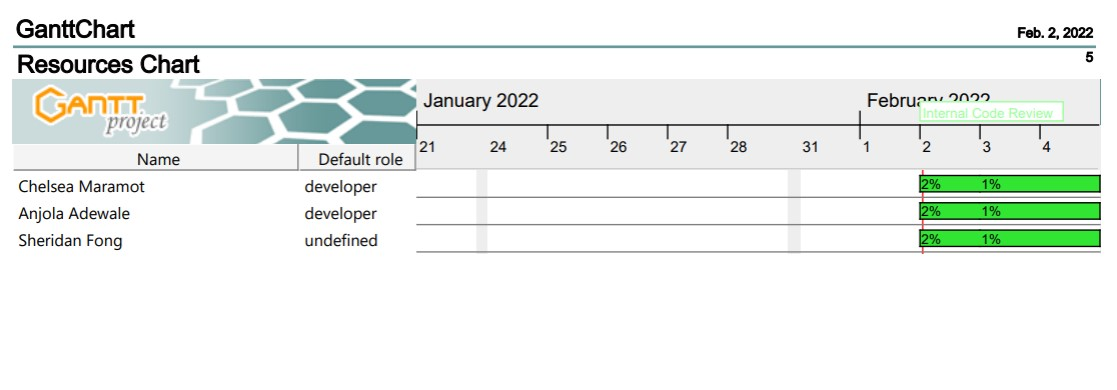
\includegraphics[scale=0.9,angle=90]{resource}
			\caption{Team Rex Resource Distribution}
		\end{figure}		
	
	
	\section{Project Review}
	
\end{document}
